\section{Cap product and ``Cech'' cohomology}

We have a few more things to say about the cap product, and will then use it
to give a statement of Poincar\'e duality. 

\begin{prop}
The cap product enjoys the following properties.\\
(1) $(a\cup b)\cap x=a\cap(b\cap x)$ and $1\cap x=x$: $H_*(X)$ is a module for
$H^*(X)$.\\
(2) Given a map $f:X\to Y$, $b\in H^p(Y)$, and $x\in H_n(X)$, 
\[
f_*(f^*(b)\cap x)=b\cap f_*(x)\,.
\]
(3) Let $\epsilon:H_*(X)\to R$ be the augmentation. Then 
\[
\varepsilon(b\cap x)=\langle b,x\rangle\,.
\]
(4) Cap and cup are adjoint:
\[
\langle a\cap b,x\rangle=\langle a,b\cap x\rangle\,.
\]
\end{prop}
\begin{proof}
(1) Easy.

\noindent
(2) Let $\beta$ be a cocycle representing $b$, and $\sigma$ an $n$-simplex
in $X$. Then
\begin{align*}
f_\ast(f^\ast(\beta)\cap\sigma)& =f_\ast(\left(f^\ast(\beta)(\sigma\circ\alpha_p)\right)\cdot(\sigma\circ\omega_q))\\
& =f_\ast(\beta(f\circ\sigma\circ\alpha_p)\cdot(\sigma\circ\omega))\\
& =\beta(f\circ\sigma\circ\alpha_p)\cdot f_\ast(\sigma\circ\omega_q)\\
& = \beta(f\circ\sigma\circ\alpha_p)\cdot(f\circ\sigma\circ\omega_q)\\
& = \beta\cap f_\ast(\sigma)
\end{align*}
This formula goes by many names: the ``projection formula,'' or ``Frobenius
reciprocity.'' 

\noindent
(3) We get zero unless $p=n$. Again let $\sigma\in\Sin_n(X)$, and compute:
\[
\varepsilon(\beta\cap\sigma)=\varepsilon(\beta(\sigma)\cdot c^0_{\sigma(n)})=\beta(\sigma)\varepsilon(c^0_{\sigma(n)})=\beta(\sigma)=\langle \beta,\sigma\rangle
\,.
\]
\end{proof}

Here now is a statement of Poincar\'e duality. It deals with the 
homological structure of compact topological manifolds. We recall the
notion of an orientation, and Theorem \ref{thm-orientation} asserting
the existence of a fundamental class $[M]\in H_n(M;R)$ in a compact
$R$-oriented $n$-manifold.

\begin{theorem}[Poincar\'e duality]
Let $M$ be a topological $n$-manifold that is compact and oriented with 
respect to a PID $R$. Then there is a unique class $[M]\in H_n(M;R)$ that
restricts to the orientation class in $H_n(M,M-a;R)$ for every $a\in M$. 
It has the property that
\[
-\cap[M]:H^p(M;R)\to H_q(M;R)\,,\quad p+q=n\,,
\]
is an isomorphism for all $p$.
\end{theorem}

You might want to go back to Lecture 25 and verify that $\RP^3\times\RP^3$
satisfies this theorem. 

Our proof of Poincar\'e duality will be by induction. In order to make the
induction go we will prove a substantially more general theorem, one that
involves relative homology and cohomology. So we begin by understanding
how the cap product behaves in relative homology.

Suppose $A\subseteq X$ is a subspace. We have:
\begin{equation*}
\xymatrix{
	0\ar[d] & & 0\ar[d]\\
	S^p(X)\otimes S_n(A)\ar[d]^{1\otimes i_\ast}\ar[r]^{i^\ast\otimes 1} & S^p(A)\otimes S_n(A)\ar[r]^-{\cap} & S_q(A)\ar[d]^{i_*}\\
	S^p(X)\otimes S_n(X)\ar[rr]^\cap\ar[d] & & S_q(X)\ar[d]\\
	S^p(X)\otimes S_n(X,A)\ar[d]\ar@{-->}[rr] & & S_q(X,A)\ar[d]\\
	0 & & 0
}
\end{equation*}
The left sequence is exact because $0\to S_n(A)\to S_n(X)\to S_n(X,A)\to 0$ splits and tensoring with $S^p(X)$ (which is not free!) therefore leaves it exact. The solid arrow diagram commutes precisely by the chain-level projection formula. There is therefore a uniquely defined map on cokernels.

This chain map yields the {\em relative cap product}
\[
\cap: H^p(X)\otimes H_n(X,A)\to H_q(X,A)
\]
It renders $ H_\ast(X,A)$ a module for the graded algebra $ H^\ast(X)$.


I want to come back to an old question, about the significance of 
relative homology. Suppose that $K\subseteq X$ is a subspace, and consider the
relative homology $H_*(X,X-K)$. Since the complement of $X-K$ in $X$ is $K$,
these groups should be regarded as giving information about $K$. If I enlarge
$K$, I make $X-K$ smaller: $K\subseteq L$ induces
$H_*(X,X-L)\to H_*(X-K)$; the relative homology is {\em contravariant}
in the variable $K$ (regarded as an object of the poset of subspaces of $X$). 

Excision gives insight into how $H_\ast(X,X-K)$ depends on $K$. 
Suppose $K\subseteq U\subseteq X$ with $\overline{K}\subseteq\mathrm{Int}(U)$. To simplify things, let's just suppose that $K$ is closed and $U$ is open.
Then $X-U$ is closed, $X-K$ is open, and $X-U\subseteq X-K$, so excision asserts that the inclusion map 
\[
H_*(U,U-K)\to H_*(X,X-K)
\]
is an isomorphism. 

The cap product puts some structure on $H_*(X,X-K)$: it's a module over 
$H^*(X)$. But we can do better! We just decided that $H_*(X,X-K)=H_*(U,U-K)$,
so the $H^*(X)$ action factors through an action by $H^*(U)$, for any open 
set $U$ containing $K$. How does this refined action change when I decrease 
$U$?
\begin{lemma}
Let $K\subseteq V\subseteq U\subseteq X$, with $K$ closed and $U,V$ open. Then:
\begin{equation*}
\xymatrix{
	 H^p(U)\ar[dd]^{i^\ast\otimes 1}\otimes H_n(X,X-K)\ar[dr]^\cap & \\
	 & H_q(X,X-K)\\
	 H^p(V)\otimes H_n(X,X-K)\ar[ur]^\cap
}
\end{equation*}
commutes.
\end{lemma}
\begin{proof}
This is just the projection formula again!
\end{proof}
Let $\mathcal{U}_K$ be the set of open neighborhoods of $K$ in $X$. It is partially ordered by reverse inclusion. This poset is directed, since the intersection of two opens is open. By the lemma, $H^p:\mathcal{U}_K\to\mathbf{Ab}$ 
is a directed system. 
\begin{definition}
The {\em \v{C}ech cohomology} of $K$ is
\[
\cHH^p(K)=\varinjlim_{U\in\mathcal{U}_K} H^p(U)\,.
\]
\end{definition}
I apologize for this bad notation; its possible dependence on the way $K$ is sitting in $X$ is not recorded. The maps in this directed systen are all maps of graded algebras, so the direct limit is naturally a commutative graded algebra. 
Since tensor product commutes with direct limits, we now get a cap product
pairing 
\[
\cap:\cHH^p(K)\otimes H_n(X,X-K)\to H_q(X,X-K)
\]
satifying the expected properties. 
This is the best you can do. It's the natural structure that this relative homology has: $ H_\ast(X,X-K)$ is a module over $\cHH^\ast(K)$.

There are compatible restriction maps $H^p(U)\to H^p(K)$, so there is a natural
map
\[
\cHH^\ast(K)\to H^\ast(K)\,.
\]
This map is often an isomorphism. Suppose $K\subseteq X$ satisfies the following ``regular neighborhood'' condition: For every open $U\supseteq K$, there exists an open $V$ with $U\supseteq V\supseteq K$ such that $K\hookrightarrow V$ is a homotopy equivalence (or actually just a homology isomorphism).
\begin{lemma} Under these conditions, $\cHH^\ast(K)\to H^\ast(K)$ is an isomorphism.
\end{lemma}
\begin{proof}
We will check that the map to $H^p(K)$ satisfies the conditions we established in Lecture 23 to be a direct limit. 

So let $x\in H^p(K)$. Let $U$ be a neighborood of $K$ in $X$ such that 
$H^p(U)\to H^p(K)$ is an isomorphism. Then indeed $x$ is in the image of
$H^p(U)$. 

Then let $U$ be a neighborhood of $K$ and let $x\in H^p(U)$ restrict to
0 in $H^p(K)$. Let $V$ be a sub-neighborood such that $H^p(V)\to H^p(K)$
is an isomorphism. Then $x$ restricts to 0 in $H^p(V)$.
\end{proof}

On the other hand, here's an example that distinguishes $\cHH^\ast$ from $H^\ast$. This is a famous example. The ``topologist's sine curve'' is the subspace of $\RR^2$ defined as follows. It is union of three
subsets, $A$, $B$, and $C$. $A$ is the graph of $\sin(\pi/x)$ where $0<x<1$.
$B$ is the interval $0\times[-1,1]$.  
$C$ is a continuous curve from $(0,-1)$ to $(1,0)$ and meeting $A\cup B$ 
only at its endpoints. 
This is a counterexample for a lot of things; you've probably seen it in 
18.901.

\medskip
\begin{center}
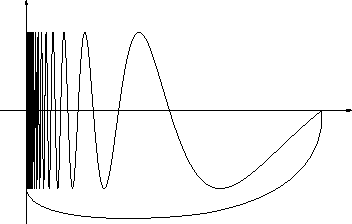
\includegraphics[width=2in]{905/Figures/34-topologists-sine-curve.pdf}
\end{center}

What is the singular homology of the topologist's sine curve? Use Mayer-Vietoris! I can choose $V$ to be some connected portion of the continuous curve from $(0,-1)$ to $(1,0)$, and $U$ to contain the rest of the space in a way that intersects $V$ in two open intervals. Then $V$ is contractible, and $U$ is made up of two contractible connected components. (This space is not locally path connected, and one of these path components is not closed.)

The Mayer-Vietoris sequence looks like
\[
0\to H_1(X)\xrightarrow{\partial} H_0(U\cap V)\to H_0(U)\oplus H_0(V)\to H_0(X)\to 0\,.
\]
The two path components of $U\cap V$ do not become connected in $U$, so $\partial=0$ and we find that $\varepsilon:H_*(X)\xrightarrow{\cong}H_*(\ast)$
and hence $H^*(X)\cong H^*(*)$. 

How about $\cHH^\ast$? Let $X\subset U$ be an open neighborhood. The interval
$0\times[-1,1]$
has an $\epsilon$-neighborhood, for some small $\epsilon$, that's contained in $U$. This implies that there exists a neighborhood $X\subseteq V\subseteq U$ such that $V\simeq S^1$. This implies that 
\[
\varinjlim_{U\in\mathcal{U}_X}H^\ast(U)\cong H^\ast(S^1)
\]
by a cofinality argument that we will detail later. So $\cHH^\ast(X)\neq H^\ast(X)$.

Nevertheless, under quite general conditions the \v{C}ech cohomology of a compact Hausdorff space is a topological invariant. The \v{C}ech construction forms
a limit over open covers of the cohomology of the nerve of the cover. It is
a topological invariant by construction. 

\begin{theorem} Let $X$ be a compact subset of some Euclidean space. If there
is an open neighborhood of which it is a retract, then $\cHH^*(X;R)$ is 
canonically isomorphic to the cohomology defined using the \v{C}ech 
construction, and is therefore independent of the embedding into Euclidean
space. 
\end{theorem}

See Dold's beautiful book \cite{dold} for this and other topics discussed
in this chapter. 
